\chapter{TINJAUAN PUSTAKA}
\label{chap:tinjauanpustaka}

% Ubah bagian-bagian berikut dengan isi dari tinjauan pustaka
\section{Penelitian Terdahulu}
\label{sec:penelitianterdahulu}

\subsection{Enhanced Vehicle Re-identification for ITS: A Feature Fusion Approach using Deep Learning}

Pada tahun 2022, Ashutosh Holla B, Manohara Pai M.M, Ujjwal Verma, dan Radhika M. Pai membuat penelitian 
re-identifikasi kendaraan. Penelitian yang mereka lakukan merupakan pengembangan sistem transportasi pintar 
yang bertujuan untuk memberikan efisiensi lalu lintas yang lebih baik dengan cara mengurangi masalah lalu 
lintas yang sering terjadi. Sistem yang mereka kembangkan merupakan sistem re-identifikasi menggunakan dua 
metode yang digabungkan, yaitu metode CNN menggunakan arsitektur ResNetmid dan metode Swin Transformer.

Pengujian dilakukan dengan melakukan re-identifikasi citra secara terpisah pada masing-masing metode, 
kemudian hasil pengujian dari tiap metode digabung sehingga menghasilkan output yang merupakan hasil 
penyatuan dari kedua metode tersebut. Pengujian menggunakan sistem yang mereka kembangkan menunjukan hasil 
yang lebih baik jika dibandingkan dengan sistem re-identifikasi tunggal masing-masing metode. Pada sistem 
ResNetmid, nilai mAP yang didapatkan sebesar 57,78. Sementara sistem Swin Transformer didapatkan mAP sebesar 
56,8. Dan pada sistem yang mereka kembangkan mendapatkan mAP sebesar 61,73\parencite{Holla2022}.

\subsection{A Vehicle Re-identification Framework Based on the Improved Multi-Branch Feature Fusion Network}

Pada tahun 2021, terdapat penelitian yang dilakukan oleh Leilei Rong, Yan Xu, Xiaolei Zhou, Lisu Han, Linghui 
Li, dan Xunghua Pan. Penelitian yang dilakukan merupakan pembuatan sistem re-identifikasi kendaraan menggunakan 
Multi-branch feature fusion network yang telah ditingkatkan. Sistem yang mereka buat bertujuan untuk memecahkan 
permasalahan dan meningkatkan akurasi dari re-identifikasi. Dengan menggunakan backbone ResNet-50 dan dataset 
dari VehicleID, VeRi-776, dan VRIC, mereka berfokus untuk meningkatkan akurasi re-identifikasi dari citra yang 
ditangkap dalam keadaan berbagai macam keadaan, seperti orientasi kendaraan ketika tertangkap kamera, keadaan 
cahaya, resolusi, blur, dan keadaan lainnya.

Dengan dilakukannya pengujian pada tiga dataset yang berbeda, didapatkan hasil bahwa model yang mereka kembangkan 
mampu melakukan re-identifikasi kendaraan dengan baik. Menggunakan dataset VehicleID, didapatkan mAP sebesar 80,87. 
Sementara  pada dataset VeRi-776, didapatkan mAP sebesar 77,12. Dan pada dataset VRIC, didapatkan mAP sebesar 
82,75\parencite{Rong2021}.

\subsection{Klasifikasi Detail Mobil Menggunakan Swin Transformer}

Pada tahun 2022, Muhammad Alif W. membuat penelitian tentang klasifikasi detail mobil menggunakan Swin Transformer. 
Sistem yang dibuat bertujuan untuk mengklasifikasikan merek dan tipe dari sebuah mobil. Dataset yang digunakan 
pada penelitian ini adalah BoxCar116K yang berisi 116 ribu citra mobil.

Peneliti membuat tiga sistem dimana pada setiap sistem menggunakan variasi model Swin Transformer dengan pengaturan 
yang berbeda. Variasi tersebut yaitu Swin-B (Swin Base), Swin-S (Swin Small), dan Swin-T (Swin Tiny). Setelah 
dilakukan pengujian, didapatkan hasil bahwa pada tiap sistem yang dibuat mampu mengklasifikasikan merek dan tipe mobil 
dengan baik. Pada sistem dengan model Swin-B, didapatkan nilai akurasinya sebesar 0,87. Sementara pada sistem dengan 
model Swin-S, didapatkan nilai akurasi sebesar 0,85. Dan pada sistem dengan model Swin-T, nilai akurasi yang didapat 
sebesar 0,84\parencite{Wicaksono2022}.

\section{Mobil}
\label{sec:mobil}

Mobil (\emph{automobile}, \emph{motorcar}, atau \emph{car}) merupakan kendaraan yang umumnya beroda empat dan dirancang untuk bergerak 
menggunakan mesin pembakaran internal menggunakan bahan bakar yang mudah menguap. Mobil memiliki sistem teknis yang 
kompleks yang terdiri dari berbagai macam subsistem yang memiliki fungsinya masing-masing. Mobil telah menjadi sarana 
utama transportasi keluarga selama bertahun-tahun, dengan perkiraan 1,4 miliar mobil beroperasi di seluruh dunia. Desain 
dari mobil Sebagian besar bergantung dari tujuan penggunaannya. Seperti misalnya mobil dengan kegunaan \emph{off-road} harus tahan 
lama terhadap kondisi medan, sistemnya sederhana namun memiliki daya tahan tinggi terhadap beban berlebih. Sementara mobil 
yang digunakan di jalan raya dengan sistem kecepatan tinggi harus memiliki kondisi seperti performa mesin yang tinggi, 
memberikan kenyamanan pada penumpang, dan mobil memiliki stabilitas yang optimal \parencite{Cromer2023}. Perbedaan 
berdasarkan fungsi dan perusahaan manufaktur membuat mobil-mobil yang ada di dunia ini memiliki ciri khasnya masing-masing 
dan dapat dibedakan satu sama lain.

\section{Citra}
\label{sec:citra}

Citra atau gambar merupakan representasi visual dari suatu objek, seperti manusia, barang, maupun pemandangan. Citra 
umumnya terbagi menjadi dua jenis, yaitu citra analog dan citra digital. Citra analog memiliki sifat kontinyu dan tidak 
dapat direpresentasikan dalam komputer sehingga tidak dapat diproses oleh komputer secara langsung \parencite{Tyagi2018}. 
Sementara citra digital merupakan sebuah larik (array) yang berisi nilai-nilai real, kompleks, dan berhingga (\emph{finite}) 
yang direpresentasikan dengan deretan bit tertentu. 

%gambar koordinat

Citra dapat didefinisikan sebagai fungsi f(x,y) berukuran M baris dan N kolom. x dan y pada fungsi merupakan koordinat 
spasial dan amplitude f di titik (x,y) adalah intensitas atau tingkat keabuan dari citra tersebut. Gambar … merupakan 
contoh sebuah koordinat citra digital \parencite{Putra2010}.

\section{\emph{Machine Learning}}
\label{sec:machinelearning}

\emph{Machine learning} (ML) merupakan salah satu disiplin dari \emph{Artificial Intelligence} (AI) dimana sebuah sistem akan 
mempelajari dan menganalisa data-data terdahulu secara otomatis. Sistem tersebut nantinya akan berfokus mengindetifikasi 
pola dari data yang telah didapat, mempelajari pola tersebut secara iteratif, kemudian membangun model berdasarkan data 
yang telah dipelajari, dan menggunakan model tersebut untuk membuat prediksi ketika diberikan sebuah data baru \parencite{Russel2021}.

Terdapat dua alasan utama perlunya membuat sebuah mesin yang dapat belajar. Alasan pertama karena pembuat mesin 
(machine designer) tidak dapat mengantisipasi seluruh kemungkinan yang ada di masa depan. Seperti misalnya sebuah robot 
yang didesain untuk menavigasikan sebuah labirin. Robot tersebut perlu mempelajari labirin tersebut sebelum dapat menavigasikannya. 
Alasan kedua yaitu karena adakalanya pembuat mesin justru tidak tahu bagaimana membuat sebuah kode untuk memecahkan permasalahan, 
sehingga menggunakan algoritma dari \emph{machine learning} untuk memecahkan masalah \parencite{Russel2021}.

\subsection{\emph{Supervised Learning}}

\emph{Supervised Learning} merupakan algoritma \emph{machine learning} yang mempelajari kumpulan input-output yang telah dipasangkan. 
Output yang telah dipasangkan ini disebut dengan label. \emph{machine learning} akan menerima beberapa input data yang telah 
dipasangkan dengan output, kemudian mempelajarinya dengan cara membandingkan output yang diperoleh dengan output yang benar. Seperti 
contohnya ketika diberikan input citra bergambar bis, maka akan memberikan output bertuliskan “bis”. Dengan \emph{Supervised Learning}, 
maka model \emph{machine learning} dapat mengklasifikasi data baru berdasarkan data training yang pernah dipelajari \parencite{Russel2021}.

\subsection{\emph{Unsupervised Learning}}

\emph{Unsupervised Learning} merupakan algoritma \emph{machine learning} yang mempelajari pola dari data yang tidak memiliki label, 
sehingga model tidak mengetahui benar atau tidaknya output yang diberikan. Umumnya \emph{Unsupervised Learning} akan mengelompokan 
(clustering) output berdasarkan contoh-contoh yang memiliki kemiripan. Contoh dari \emph{Unsupervised Learning} yaitu Ketika memberikan 
input citra bergambar kucing, maka model akan memberikan output berbagai macam citra yang memiliki kemiripan atau berhubungan dengan 
kucing \parencite{Russel2021}.

\section{\emph{Deep Learning}}
\label{sec:deeplearning}

\emph{Deep Learning} merupakan salah satu cabang dari \emph{machine learning} (ML) dimana model yang dibuat untuk mendapatkan output 
mengikuti bentuk model neuron dari otak manusia, sehingga sering juga disebut dengan \emph{neural network}. Metode \emph{Deep Learning} 
memiliki bentuk rangkaian yang memiliki banyak layer di dalamnya, sehingga data yang masuk akan melalui sejumlah layer yang telah ditetapkan 
hingga menjadi sebuah output. Tidak seperti metode lainnya yang dapat menangani banyak data dan memiliki waktu proses yang singkat, proses 
menggunakan metode \emph{Deep Learning} bergantung dari jumlah layer yang digunakan di dalam model. Semakin banyak layer yang digunakan mengakibatkan 
waktu untuk memproses data lebih lama karena tingkat kompleksitas yang semakin tinggi. Metode \emph{Deep Learning} banyak diaplikasikan pada 
\emph{visual object recognition}, \emph{machine translation}, \emph{speech recognition}, \emph{speech synthesis}, dan \emph{image synthesis} 
\parencite{Russel2021}.

%gambar

\emph{Deep Learning} terbukti memiliki keunggulan yang lebih dibandingkan menggunakan \linebreak metode lainnya, khususnya data yang memiliki dimensi 
tinggi seperti citra. Seperti misalnya pada metode linear dan metode linear regression, kedua metode tersebut dapat menangani variabel input 
yang cukup besar, namun ketika dilakukan perhitungan, waktu yang dibutuhkan cukup singkat, karena setiap variabel input yang berbeda hanya 
berhubungan secara independen dengan output. Setiap variabel input ini tidak memiliki keterhubungan satu sama lain. Sifat dari metode ini 
menyebabkan model yang dihasilkan terbatasi kemampuannya. Model yang dihasilkan hanya sebatas mengikuti fungsi linear dan batas yang ada di 
bagian input. Dimana pada dunia nyata, konsep dan input yang harus diolah lebih kompleks. Hal inilah yang membuat \emph{Deep Learning} memiliki 
keunggulan yang signifikan. Gambar … merupakan contoh perbandingan dari jaringan komputasi yang dimiliki oleh metode \emph{linear regression}, metode 
\emph{decision list network}, dan metode \emph{deep learning} \parencite{Russel2021}. 

\section{\emph{Re-identifikasi}}
\label{sec:re-identifikasi}

Re-identifikasi merupakan teknik mencocokan dua objek dengan bidang pandang berbeda berdasarkan kemiripan pada beberapa parameter yang telah 
ditentukan dengan tujuan untuk membuktikan bahwa kedua objek tersebut sama. Karakteristik dari re-identifikasi berupa sebuah siklus hipotesis-deduktif, 
dimana model prediksi yang dibuat dengan mempelajari training data akan mengumpulkan data baru dari masukan, kemudian diikuti dengan revisi dan 
pelabelan baru untuk data yang memiliki nilai kecocokan tinggi. Hal tersebut akan terus berulang mengikuti data terbaru yang dimasukan ke model 
prediksi tersebut \parencite{Wechsler2014}.

%gambar

Kebutuhan akan adanya sebuah sistem re-identifikasi dikaitkan dengan beberapa alasan, seperti untuk meningkatkan keamanan di lingkungan publik 
yang menyebabkan penyebaran kamera CCTV yang meluas di area seperti taman, kampus, sekolah, jalan raya, dan lainnya. Semakin banyaknya kamera CCTV 
di lingkungan publik berbanding lurus dengan semakin banyaknya tenaga kerja kasar manusia yang dibutuhkan untuk melihat dan melacak orang/kendaraan 
secara akurat dan efisien melalui kamera \parencite{Zheng2016}. Semakin sulitnya melakukan re-identifikasi secara manual menjadi alasan kuat perlu dikembangkannya 
sistem re-identifikasi yang akurat dan efisien.

\section{Transformer}
\label{sec:transformer}

Model transduksi urutan dominan (\emph{dominant sequence transduction model}) yang ada diciptakan menggunakan arsitektur \emph{convolutional neural network} 
(CNN) atau \emph{recurrent neural network} (RNN) kompleks, yang memiliki encoder dan decoder. Namun pada 2017, diperkenalkan arsitektur jaringan yang cukup 
simpel, yang disebut The Transformer. Arsitektur Transformer memperkenalkan sebuah sistem jaringan saraf yang berfokus pada mekanisme perhatian (\emph{attention}) 
dengan bantuan encoder dan decoder, tanpa menggunakan \emph{reccurent network} dan konvolusi seperti yang ada pada model \emph{sequence to sequence}. 

Ketika diperkenalkan,Transformer diuji cobakan untuk menjadi sebuah model penerjemah Bahasa. Ketika dibandingkan dengan model ber-asitektur CNN dan RNN 
(seperti Extended Neural GPU, ByteNet, dan ConvS2S), terbukti bahwa Transformer, sebuah arsitektur tanpa RNN dan hanya menggunakan mekanisme perhatian, dapat 
melakukan training lebih cepat dengan training data yang terbatas dan ukuran yang besar, serta skor output training yang dihasilkan pun juga mengungguli model-model 
ber-asitektur CNN dan RNN. \parencite{Vaswani2017}

\section{Swin Transformer}
\label{sec:swintransformer}

Pemodelan pada visi komputer telah lama didominasi oleh \emph{Convolutional Neural Network} (CNN), dimulai dengan AlexNet dan kinerja revolusinya di tantangan 
klasifikasi gambar ImageNet. Arsitektur CNN telah berevolusi menjadi arsitektur yang hebat dengan skala yang lebih besar, koneksi yang lebih luas, dan bentuk 
konvolusinya yang lebih canggih. Sementara arsitektur Transformer yang saat ini lazim digunakan pada \emph{Natural Language Processing} (NLP), justru tidak cocok 
ketika digunakan sebagai model pada visi komputer. Hal ini dikarenakan pada tugas visi komputer seperti segmentasi semantik, dibutuhkan fitur prediksi hingga pada 
tingkat piksel. Hal ini cukup sulit untuk arsitektur Transformer ketika dihadapkan gambar beresolusi tinggi, karena mekanisme kompleksitas komputasi \emph{self-attention} 
yang dimiliki bersifat kuadratik terhadap ukuran gambar. Sehingga untuk mengatasi masalah tersebut, diciptakanlah Swin Transformer. \parencite{Liu2021}

%gambar

Swin Transformer sebagai sebuah arsitektur baru untuk visi komputer, mampu \linebreak memetakan hirarki dan kompleksitas komputasinya mengikuti ukuran gambar. Seperti yang 
terlihat pada gambar … , Swin Transformer membangun sebuah hirarkis dengan \emph{patch} berukuran kecil (bergaris abu-abu) pada lapisan atas, yang kemudian secara 
bertahap \emph{patch} tersebut akan bergabung dengan sekitarnya di lapisan yang lebih dalam. Selain itu, Swin Transformer memiliki kompleksitas komputasi yang linear 
terhadap ukuran gambar dikarenakan komputasi \emph{self-attention} hanya berfokus pada setiap jendela (bergaris merah). Berbeda dengan Vision Transformer yang 
memetakan dengan resolusi rendah dan memiliki kompleksitas komputasi kuadratik terhadap ukuran gambar karena komputasi \emph{self-attention} dilakukan secara 
menyeluruh. \parencite{Liu2021}

\subsection{\emph{Shifted Windows}}

Arsitektur standar Transformer dan adaptasinya untuk klasifikasi gambar menggunakan \emph{global self-attention}. \emph{global self-attention} merupakan hubungan antara 
satu token dengan token lainnya ketika dikomputasikan. Perhitungan global ke kompleksitas kuadrat berhubungan dengan jumlah token. Hal ini membuat Transformer tidak cocok 
untuk menyelesaikan permasalahan visi yang membutuhkan kumpulan token yang besar untuk prediksi padat pada gambar beresolusi tinggi. \parencite{Liu2021}

%gambar

Karenanya, diciptakanlah \emph{shifted windows} untuk memperbaiki kekurangan dari \linebreak transformer. Gambar … merupakan sebuah ilustrasi dari pendekatan \emph{shifted windows} 
untuk menghitung \emph{self-attention} yang dikenalkan pada arsitektur Swin Transformer. Pada layer 1 (kiri), skema partisi dari jendela biasa diadopsi, dan \emph{self-attention} 
akan dihitung pada setiap jendelanya. Kemudian pada layer \begin{math}1+1\end{math} (kanan), jendela partisi akan bergeser (\emph{shifted}) dan menghasilkan jendela baru. Perhitungan 
\emph{self-attention} di jendela yang baru melintasi Batasan dari jendela sebelumnya di layer 1, dimana menyediakan koneksi diantaranya. \parencite{Liu2021}

\subsection{Arsitektur Swin Transformer}

%gambar

Gambaran dari arsitektur Swin Transformer dapat dilihat pada gambar …, yang mengilustrasikan versi kecil dari Swin Transformer (Swin-T). Pada tahap awal, gambar input akan 
dibagi menjadi \emph{patch} non-tumpang tindih menggunakan modul pemecah tambalan, seperti ViT. Setiap \emph{patch} yang dihasilkan diperlakukan sebagai “token” dan fiturnya ditetapkan sebagai 
rangkaian dari nilai RGB piksel mentah. Dalam implementasinya, ukuran \emph{patch} yang digunakan adalah \begin{math}4 \times 4\end{math}, sehingga dimensi fitur dari masing-masing \emph{patch} adalah 
\begin{math}4 \times 4 \times 3 = 48\end{math}. Lapisan linear diterapkan pada fitur bernilai mentah ini untuk memproyeksikannya ke sembarang dimensi (dilambangkan sebagai C). \parencite{Liu2021}

Beberapa blok Transformer dengan perhitungan \emph{self-attention} yang dimodifikasi diterapkan pada token \emph{patch} ini. Blok Transformer mempertahankan jumlah tokennya 
(\begin{math}\frac{H}{4} \times \frac{H}{4}\end{math}), dan bersama dengan penyematan linear disebut dengan “tahap 1”. \parencite{Liu2021}

Untuk menghasilkan representasi hierarkis, semakin dalamnya jaringan akan membuat jumlah token dikurangi dengan lapisan yang menggabungkan \emph{patch}. Lapisan penggabungan \emph{patch} pertama menggabungkan 
fitur dari setiap kelompok \emph{patch} sekitarnya \begin{math}2 \times 2\end{math}, yang kemudian diterapkan di lapisan linear pada rangkaian fitur dimensi 4C. Hal ini mengurangi jumlah token dengan 
kelipatan \begin{math}2 \times 2 = 4\end{math} (\begin{math}2 \times resolusi downsampling\end{math}), dan dimensi keluarannya diatur ke 2C. Blok Swin Transformer diterapkan setelahnya untuk 
transformasi fitur, dengan resolusi tetap pada \begin{math}\frac{H}{8} \times \frac{W}{8}\end{math}. Blok penggabungan patch pertama yang ditambah dengan transformasi fitur dinotasikan sebagai 
“tahap 2”. Kemudian prosedur ini diulang dua kali, sebagai “tahap 3” dan “tahap 4”, dengan resolusi keluaran dari \begin{math}\frac{H}{16} \times \frac{W}{16}\end{math} dan 
\begin{math}\frac{H}{32} \times \frac{W}{32}\end{math}. Tahapan-tahapan ini menghasilkan representasi hierarkis, dengan resolusi peta fitur yang sama dengan jaringan konvolusional. \parencite{Liu2021}

\subsection{Blok Swin Transformer}

%gambar

Swin Transformer dibangun dengan menggantikan standar modul \emph{multi-head self attention} (MSA) di dalam blok Transformer dengan modul \emph{shifted windows} (dijelaskan pada bagian …), dengan 
lapisan lain tetap sama. Seperti yang diilustrasikan pada gambar …, blok Swin Transformer terdiri dari \emph{shifted windows} dengan basis modul MSA, yang kemudian diikuti 2 layer MLP dengan 
nonlinear GELU diantaranya. Lapisan \emph{LayerNorm} (LN) diterapkan sebelum setiap modul MSA dan MLP, dan residu koneksi diterapkan di setiap setelah modul. \parencite{Liu2021}

\subsection{Variasi Model}

Swin Transformer memiliki beberapa variasi model yang dapat digunakan. Swin-B (\emph{Swin Base}) dibuat dengan ukuran model dan tingkat kompleksitas komputasi yang mirip dengan ViT-B 
(\emph{Vision Transformer Base}). Selain itu, dikenalkan juga varian model Swin-T, Swin-S, dan Swin-L. Swin-T (\emph{Swin Tiny}) merupakan versi 0.25x ukuran dan tingkat kompleksitas 
komputasi dari \emph{base}. Swin-S (\emph{Swin Small}) merupakan versi 0.5x dari \emph{base}, sementara Swin-L (\emph{Swin Large}) merupakan versi 2x dari \emph{base}. Swin-T dan Swin-S 
memiliki kompleksitas yang mirip dengan ResNet-50 dan ResNet-101. Ukuran jendela diatur ke M = 7 secara default. Sementara dimensi kueri pada setiap kepala adalah d = 32, dan lapisan 
ekspansi di setiap MLP adalah \begin{math}\alpha = 4\end{math}, untuk semua parameter. Hyper-parameter dari setiap variasi modelnya adalah sebagai berikut:

\begin{itemize}[nolistsep]

  \item Swin-T: C = 96, jumlah layer = {2, 2, 6, 2}

  \item Swin-S: C = 96, jumlah layer = {2, 2, 18, 2}

  \item Swin-B: C = 128, jumlah layer = {2, 2, 18, 2}

  \item Swin-L: C = 192, jumlah layer = {2, 2, 18, 2}

\end{itemize}

C merupakan nomor saluran dari lapisan tersembunyi di tahap pertama. \parencite{Liu2021}

Setelah dilakukan percobaan di 3 jenis tugas, hasil percobaan menunjukan bahwa Swin Transformer memiliki performa yang bagus untuk digunakan di tugas visi. Hal ini dikarenakan pada klasifikasi gambar, Swin 
Transformer mendapatkan akurasi 84,5 pada ImageNet-1K dan akurasi 87,3 pada ImageNet-22K pre-trained models. Kemudian pada deteksi objek, Swin Transformer mendapatkan nilai 58,7 untuk box AP dan 51,1 
untuk mask AP pada pengembangan deteksi objek COCO. Dan pada segmentasi semantik, Swin Transformer mendapatkan nilai 53.5 untuk mIoU pada ADE20K. Hal ini menunjukan bahwa Swin Transformer memiliki potensi 
untuk menjadi basis di tugas visi. \parencite{Liu2021}

\section{Swin Transformer V2}
\label{sec:swintransformerv2}



\section{VRIC Dataset}
\label{sec:vricdataset}

Selama dua tahun terakhir, re-identifikasi kendaraan menjadi perhatian dikarenakan memiliki potensi untuk lebih fleksibel dalam melakukan pengenalan dan pencarian kendaraan dibandingkan 
menggunakan \emph{Automatic Number Plate Recognition} (ANPR). Walaupun begitu, re-identifikasi kendaraan berdasarkan penampilan visual menjadi tantangan tersendiri dikarenakan kemungkinan 
kendaraan memiliki penampilan yang sangat mirip dimana kendaraan yang berbeda namun jenis dan warna, model yang sama serta visual model yang bervariasi berdasarkan posisi pengambilan 
gambar. Studi re-identifikasi kendaraan yang ada umumnya menggunakan salah satu dari dua dataset ini, yaitu VehicleID dan VeRi-776. Walaupun hasil studi menunjukkan hasil cukup memuaskan, 
namun pengaplikasian di dunia nyata belum jelas, dikarenakan dataset yang digunakan menggunakan gambar berkualitas tinggi dengan resolusi tinggi, tidak ada \emph{motion blur}, kondisi cuaca 
khusus, dan oklusi. Karena alasan inilah, diciptakan sebuah dataset baru yaitu \emph{Vehicle Re-Identification in Context} (VRIC). Perbedaan dataset antara VehicleID, VeRi-776, dan VRIC 
dapat dilihat pada gambar … \parencite{Kanaci2018}

%gambar

VRIC merupakan dataset yang lebih realistis dan menantang yang dikhususkan untuk re-identifikasi kendaraan. VRIC berisikan 60.430 gambar dengan 5.622 ID kendaraan yang diambil dari 60 
kamera lalu lintas yang berbeda. VRIC berbeda dengan dataset dua dataset lainnya karena gambar yang diambil memiliki resolusi gambar yang bervariasi, terdapat \emph{motion blur}, kondisi 
cuaca yang bermacam-macam, dan oklusi. Hal ini membuat VRIC dapat memberikan benchmark dari re-identifikasi kendaraan yang lebih realistis. \parencite{Kanaci2018}

\subsection{Sumber Gambar}

Karena terdapat keterbatasan dalam pengaksesan data video pengawasan, sehingga VRIC menggunakan set data kendaraan yang tersedia untuk umum yang disediakan oleh komunitas riset. Sumber 
data kendaraan diambil dari UA-DETRAC \emph{object detection and tracking benchmark} dengan pertimbangan sebagai berikut:

\begin{itemize}[nolistsep]

  \item Seluruh video ditangkap dari adegan lalu lintas yang berada di dunia nyata, mencerminkan konteks “realistis” untuk re-identifikasi kendaraan.

  \item Video yang ada mencakup 24 lokasi penangkapan yang berbeda dengan kondisi lingkungan yang beragam, sehingga menawarkan skenario pengujian yang kaya tanpa bias terhadap kondisi 
  tertentu. 

  \item Berisi anotasi objek dan atribut yang kaya yang dapat memfasilitasi pelabelan ID untuk re-identifikasi kendaraan.

\end{itemize}

%gambar

Contoh tangkapan gambar lalu lintas dan \emph{bounding-box} kendaraan dapat dilihat pada gambar … \parencite{Kanaci2018}

\subsection{Filter dan Anotasi Gambar}

Dataset VRIC dibuat dengan menggunakan 60 training video dengan anotasi objek \emph{bounding-box} yang berasal dari UA-DETRAC. Anotasi identitas kendaraan (ID) dilakukan dengan menetapkan 
label unik untuk setiap lintasan kendaraan per video UA-DETRAC, kemudian memverifikasi duplikasi ID secara manual. Dikarenakan seluruh video mentah UA-DETRAC diambil dari waktu dan adegan 
yang berbeda, ditemukan sedikit lintasan duplikat dalam hal identitas. Untuk membuat cukup banyak variasi tampilan kendaraan, maka dibuanglah lintasan pendek yang memiliki kurang dari 20 
frame, dan \emph{bounding-box} yang lebih kecil dari \begin{math}24 \times 24\end{math}. Sehingga dengan dilakukannya hal tersebut, didapatkan 5.622 ID kendaraan dari keseluruhan 60 video. 
\parencite{Kanaci2018}

%gambar

Seperti yang terlihat di gambar …, rata-rata resolusi gambar dari 60.430 \emph{bounding-box} kendaraan adalah \begin{math}69,8 \times 107,5\end{math} piksel pada 
\begin{math}lebar \times tinggi\end{math}, dengan variasi 32 hingga 280 piksel dikarenakan jarak yang tidak dibatasi antara kendaraan dan kamera. \parencite{Kanaci2018}

\subsection{Splitting Dataset}

Untuk model \emph{training} dan \emph{testing} menggunakan VRIC dataset sebagai benchmark, 5.622 ID kendaraan dari VRIC dibagi secara acak menjadi dua dan tidak tumpang tindih, dengan 
2.811 untuk \emph{training}, dan 2.811 untuk \emph{testing}. Karena tidak ada pencocokan ID berpasangan lintas kamera, maka disimulasikan variasi tampilan silang dengan pengambilan 
sampel jarak jauh antara gambar \emph{probe} dan \emph{gallery}. \parencite{Kanaci2018} Pembagian data untuk kebutuhan \emph{training} dan \emph{testing} dapat dilihat pada gambar …

%gambar

Secara khusus, VRIC memiliki dua tampilan semu, yaitu dekat atau jauh, untuk setiap video dan kemudian akan dibangun set \emph{probe/gallery} dari lintasan uji dengan mengambil sampel 
dari dua tampilan semu tersebut secara acak. Tampilan jarak jauh dan dekat ini menghasilkan kondisi yang sangat berbeda dan memungkinkan untuk digunakan pada simulasi dari dua pandangan 
kamera yang tidak tumpang tindih. \parencite{Kanaci2018}


% % Contoh input gambar
% \begin{figure}[ht]
%   \centering

%   % Ubah dengan nama file gambar dan ukuran yang akan digunakan
%   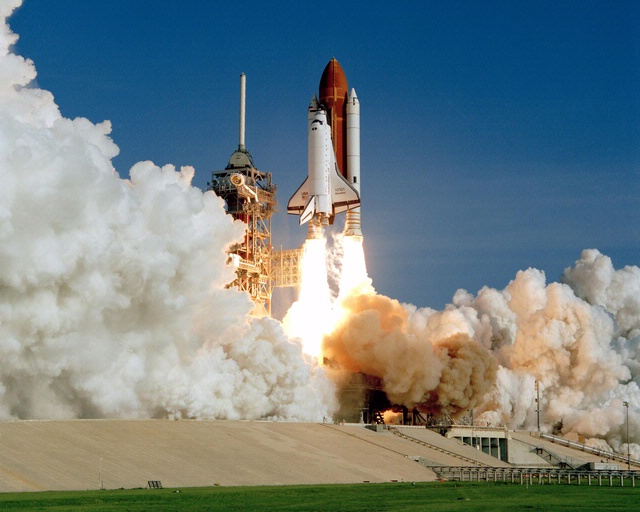
\includegraphics[scale=0.35]{gambar/roketluarangkasa.jpg}

%   % Ubah dengan keterangan gambar yang diinginkan
%   \caption{Peluncuran roket luar angkasa \emph{Discovery} \parencite{roketluarangkasa}.}
%   \label{fig:roketluarangkasa}
% \end{figure}

% Roket luar angkasa merupakan \lipsum[1]

% \emph{Discovery}, Gambar \ref{fig:roketluarangkasa}, merupakan \lipsum[2]

% \section{Gravitasi}
% \label{sec:gravitasi}

% Gravitasi merupakan \lipsum[1]

% \subsection{Hukum Newton}
% \label{subsec:hukumnewton}

% Newton \parencite{newton1687} pernah merumuskan bahwa \lipsum[1]
% Kemudian menjadi persamaan seperti pada persamaan \ref{eq:hukumpertamanewton}.

% % Contoh pembuatan persamaan
% \begin{equation}
%   \label{eq:hukumpertamanewton}
%   \sum \mathbf{F} = 0\; \Leftrightarrow\; \frac{\mathrm{d} \mathbf{v} }{\mathrm{d}t} = 0.
% \end{equation}

% \subsection{Anti Gravitasi}
% \label{subsec:antigravitasi}

% Anti gravitasi merupakan \lipsum[1]
